\documentclass{article}
\usepackage[margin=1in]{geometry}
\usepackage{amsmath,amsthm,amssymb}
\usepackage{bbm,enumerate,mathtools}
\usepackage{tikz,pgfplots}
\usepackage{chessboard}
\usepackage[hidelinks]{hyperref}
\usepackage{multicol} % Problem 35

\newenvironment{question}{\begin{trivlist}\item[\textbf{Question.}]}{\end{trivlist}}
\newenvironment{note}{\begin{trivlist}\item[\textbf{Note.}]}{\end{trivlist}}
\newenvironment{references}{\begin{trivlist}\item[\textbf{References.}]}{\end{trivlist}}
\newenvironment{related}{\begin{trivlist}\item[\textbf{Related.}]\end{trivlist}\begin{enumerate}}{\end{enumerate}}


\begin{document}
\rating{2}{3}
Consider ways to place colored markers on an $n \times m$ grid so that no two
pairs of markers of the same color have the same distance between them.

\begin{figure}[!h]
  \centering
  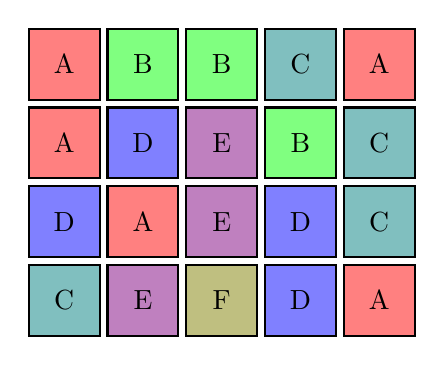
\begin{tikzpicture}
    \def\polyomino{
      0/3/1/0/0/1/A, 1/3/0/1/0/1/B, 2/3/0/1/0/1/B, 3/3/0/1/1/2/C, 4/3/1/0/0/1/A,
      0/2/1/0/0/1/A, 1/2/0/0/1/1/D, 2/2/1/0/1/2/E, 3/2/0/1/0/1/B, 4/2/0/1/1/2/C,
      0/1/0/0/1/1/D, 1/1/1/0/0/1/A, 2/1/1/0/1/2/E, 3/1/0/0/1/1/D, 4/1/0/1/1/2/C,
      0/0/0/1/1/2/C, 1/0/1/0/1/2/E, 2/0/1/1/0/2/F, 3/0/0/0/1/1/D, 4/0/1/0/0/1/A
    }
    \foreach \x/\y/\r/\g/\b/\w/\l in \polyomino {
      \draw[thick,fill={rgb:red,\r;green,\g;blue,\b;white,\w}]
        (\x - 0.45, \y - 0.45) rectangle (\x + 0.45, \y + 0.45) node[pos=.5] {\l};
    }
  \end{tikzpicture}\\
  \caption{
    This arrangement has $6$ different colors of markers.
    There are $5$ red (A) markers and no valid way to place $6$ red markers.
  }
\end{figure}

\begin{question}
  What is $c_{n \times m}$ the greatest number of markers of a given color can
  be placed on the $n \times m$ grid?
\end{question}
\begin{related}
  \item How many colors of markers are required to fill the grid?
  \item What if this is done on the $d_1$, $d_\infty$, or $d_3$ metric?
  \item What if this is done on a triangular or hexagonal grid?
  \item What is the smallest board that can contain $k$ markers?
\end{related}
\begin{note}
  $c_{n \times m}(c_{n \times m}-1)/2 \leq A301853(n, m) - 1.$
\end{note}
\begin{references}
  \item Problem 30.
  \item \url{https://oeis.org/A301853}
\end{references}
\end{document}
